\documentclass[11pt]{article}

\usepackage[preprint]{acl}

\usepackage{times}
\usepackage{latexsym}

\usepackage[T1]{fontenc}
\usepackage[utf8]{inputenc}

\usepackage{microtype}
\usepackage{inconsolata}
\usepackage{graphicx}
\usepackage{amsmath}
\usepackage{amssymb}
\usepackage{booktabs}
\usepackage{array}
\usepackage{soul}
\usepackage{enumitem}
\usepackage{tikz}
\usepackage{stfloats}
\usepackage{float}
\usetikzlibrary{positioning,arrows.meta}

\newcommand{\mask}{\ensuremath{\mathrm{m}}}
\newcommand{\keep}{\textsc{keep}}
\newcommand{\edit}{\textsc{edit}}
\newcommand{\drop}{\textsc{drop}}
\newcommand{\maskdisc}{\textsc{[mask]-disc}}
\newcommand{\Tau}{\mathrm{T}}
% example cards in the appendix: pastel fills of the figure palette
\definecolor{exmask}{HTML}{D7DADF}
\definecolor{exok}{HTML}{B7DEC3}
\definecolor{exbad}{HTML}{F2B8B5}
\newcommand{\hlmask}[1]{{\sethlcolor{exmask}\hl{#1}}}
\newcommand{\hlok}[1]{{\sethlcolor{exok}\hl{#1}}}
\newcommand{\hlbad}[1]{{\sethlcolor{exbad}\hl{#1}}}
\newcommand{\stline}[2]{\par\noindent\hangindent=1.3em\hangafter=1\makebox[1.3em][l]{#1}#2}
\newcommand{\exrow}[3][]{\par\noindent\hangindent=6.6em\hangafter=1\makebox[6.6em][l]{#2}#3\ifx&#1&\else~#1\fi}

\title{DiffusEdit: Mid-submission \\ Team Wordsmiths}

\author{
  \textbf{Tatva Agarwal\textsuperscript{*}} \\ 2024117005 \And
  \textbf{Vedant Kulkarni\textsuperscript{*}} \\ 2024101140 \And
  \textbf{Bysani Veda Vyas\textsuperscript{*}} \\ 2024101025 \And
  \textbf{Venya Velmurugan\textsuperscript{*}} \\ 2024114002
}

\begin{document}

\maketitle

\renewcommand{\thefootnote}{\fnsymbol{footnote}}
\footnotetext[1]{Equal contribution; authors listed alphabetically.}
\renewcommand{\thefootnote}{\arabic{footnote}}
\setcounter{footnote}{0}

\begin{abstract}
    Reference articles go out of date as events develop, and updating them by hand is slow. Regenerating the article with a language model automates the update, but rewrites text that was already correct and leaves no record of what changed. DiffusEdit instead edits the article in place.\footnote{\url{https://github.com/gamemaker1/diffusedit}} Small trained layers, reading the hidden states of a frozen masked diffusion language model, decide which sentences to keep, edit, or delete, and which tokens inside them are stale. The frozen model rewrites only the stale positions, and the system repeats the process on sentences that the rewrites themselves made wrong. Training labels come from pairs of Wikipedia snapshots, and evaluation measures update quality, faithfulness, minimality, and coverage of the cascading edits.
\end{abstract}

\section{Introduction}
    Reference text goes out of date. A Wikipedia article about a factory fire may say that three people died and that the small death toll limited the political fallout. A week later, news reports revise the toll to forty-two. The first sentence is contradicted directly, but the second is wrong since it depends on a fact that no longer holds. We call the second kind of required change a \emph{cascading edit}, a sentence that must change only because another sentence changed.
    
    DiffusEdit updates the article in place. Small trained heads over a frozen masked diffusion model choose the stale sentences and tokens, the model infills only those positions, and the loop repeats on sentences the repairs themselves broke. On the fire example, round one masks \emph{three} and infills \emph{forty-two}, and round two rewrites the fallout sentence the first repair left unsupported.
    
\section{Task Definition}
\label{sec:problem}

    An article is a sequence of sentences $A = (s_1, \dots, s_n)$, new evidence arrives as a set of text snippets $E = (e_1, \dots, e_m)$, and the system must produce an updated article $\hat{A}$ from the two alone. Faithfulness requires every claim in $\hat{A}$ to agree with the evidence and the untouched parts of the article, coverage requires every evidence fact that bears on the article to appear in $\hat{A}$, and minimality requires $\hat{A}$ to stay close to $A$.

\section{Related Work}
\label{sec:related}

    Early evidence-driven correction handles one sentence or claim at a time, masks the tokens that a new fact contradicts and refills them \citep{shah-etal-2020-automatic, thorne-vlachos-2021-evidence}. Closest to us, FRUIT \citep{iv-etal-2022-fruit} defines the task this project works on, and its EDIT5 model writes the updated article left to right while copying unchanged sentences through special tokens.
    
    EditPropBench \citep{kruthof-2026-editpropbench} measures how many required downstream changes a model finds after a planted edit, and the strongest prompted model tested misses about 30\% of them when the dependence is implicit. HiCaM \citep{shi-etal-2025-hicam} propagates a change by having a prompted model build an entity graph and a summary tree of the document.
    
    In diffusion decoding, several works reconsider tokens the sampler already committed \citep{wang-etal-2025-remasking, bie-etal-2026-llada21}. \citet{yao-2026-remask} argue for re-masking such tokens instead of overwriting them, and we reuse their per-position re-masking cap. Detect, Remask, Repair \citep[DRR;][]{zou-etal-2026-detect} is a prior system that applies a diffusion model to existing text and external evidence. It scores each token of a stale summary with \maskdisc{}, a linear classification head over the diffusion model's hidden states, then masks and infills the highest-scoring tokens, re-scoring the summary over several rounds. Our work extends this system.

\section{Motivation}
\label{sec:motivation}

The shortcomings of existing work are as follows.

    \emph{Cascades are not modeled.} DRR detects tokens that clash with the evidence, on summaries of about ninety tokens. A cascading edit clashes only with another sentence that changed, so scoring against the evidence has no signal for it, and nothing in the design tracks which sentences depend on which.
    
    \emph{Infilling cannot delete.} Every mask must be filled by exactly one token, so a system built on infilling alone can rewrite a sentence but never remove it.
    
    \emph{No token-level supervision exists.} FRUIT pairs outdated and updated articles without labeling which tokens went stale, and DRR trains on short synthetic summaries, so article-scale training data must be derived.
   
\section{Methodology and Current Progress}
  %^ pipeline image
    \begin{figure}[t]
    \centering
    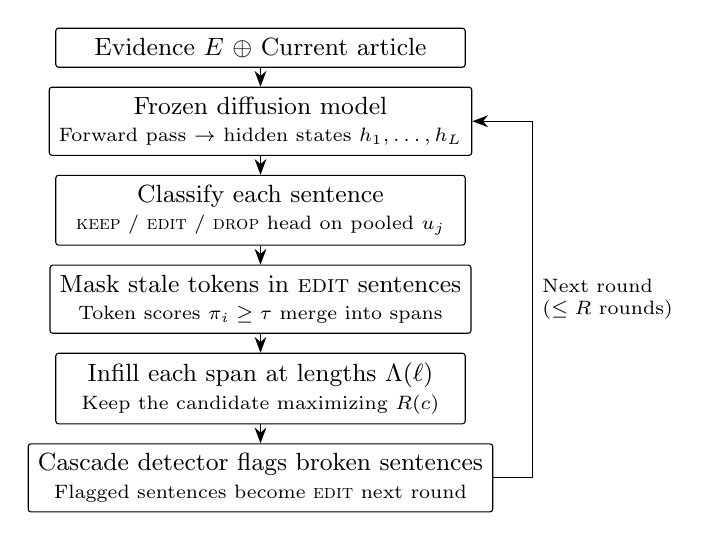
\begin{tikzpicture}[
  node distance=2.4mm,
  box/.style={draw, rounded corners=1pt, align=center, font=\small, inner sep=3.5pt, minimum width=5.2cm},
  >={Stealth[length=2mm]}
]
\node[box] (input) {Evidence $E$ $\oplus$ Current article};
\node[box, below=of input] (model) {Frozen diffusion model\\[-1pt] {\scriptsize Forward pass $\rightarrow$ hidden states $h_1, \dots, h_L$}};
\node[box, below=of model] (cls) {Classify each sentence\\[-1pt] {\scriptsize \keep{} / \edit{} / \drop{} head on pooled $u_j$}};
\node[box, below=of cls] (mask) {Mask stale tokens in \edit{} sentences\\[-1pt] {\scriptsize Token scores $\pi_i \ge \tau$ merge into spans}};
\node[box, below=of mask] (infill) {Infill each span at lengths $\Lambda(\ell)$\\[-1pt] {\scriptsize Keep the candidate maximizing $R(c)$}};
\node[box, below=of infill] (casc) {Cascade detector flags broken sentences\\[-1pt] {\scriptsize Flagged sentences become \edit{} next round}};
\draw[->] (input) -- (model);
\draw[->] (model) -- (cls);
\draw[->] (cls) -- (mask);
\draw[->] (mask) -- (infill);
\draw[->] (infill) -- (casc);
\draw[->] (casc.east) -- ++(5mm,0) |- (model.east)
  node[pos=0.25, right, font=\scriptsize, align=left] {Next round\\($\le R$ rounds)};
\end{tikzpicture}
    \caption{One round of DiffusEdit.}
    \label{fig:pipeline}
    \end{figure}
\label{sec:progress}
    We keep the LLaDA-8B model frozen while training the light weight heads (linear classifier) on pooled hidden states extracted from that model.
    \subsection{Data Processing and Feature Extraction}
    \label{subsec:data}
    Each FRUIT record lists the source sentences, the evidence snippets, and a target that copies some source sentences and writes new text for the rest. We split the new text into sentences with spaCy. We drop an instance if its article exceeds 400 LLaDA tokens, or if no source sentence is edited or deleted, because an update that only adds sentences needs an insertion step the design does not have. Of 102,902 training instances, 77,432 remain. Of 11,561 dev instances, 8,685 remain. A seeded draw takes 2,000 of these as the validation split, and the other 6,685 join training, so the training split holds 84,117 articles. The gold test set keeps 730 of its 914 instances.

    A greedy aligner pairs source and target sentences. The similarity of two sentences is the F1 overlap of their lowercased token multisets. The aligner accepts pairs in order of decreasing similarity, uses each sentence at most once, and stops below 0.35. An unpaired source sentence is \drop{}. A paired sentence is \keep{} if its similarity is at least 0.95 and no changed word contains a capital letter or a digit, and \edit{} otherwise. The capital-or-digit test, which we call the \keep{} fix, is a cheap proxy for a changed name or number, and it moved 7,991 sentences with a one-word change such as a new club or year from \keep{} to \edit{}. The training split holds 174,873 \keep{}, 162,053 \edit{} and 47,862 \drop{} sentences.

    For each \edit{} sentence, a word-level diff against its partner (Python's \texttt{difflib}) marks replaced and deleted source tokens stale. An insertion marks the token before it, so that a mask at that position can grow into the inserted text.

    The evidence of one article may hold at most 600 LLaDA tokens. Snippets enter in order of the number of mentions they share with the article, and the first snippet that does not fit is cut to fit. In the training split, 45.6\% of articles lose evidence this way, and 14.9\% of the 516,999 snippets end up empty. These articles lose a median 25.4\% of their evidence characters, and in 13.1\% of all training articles a snippet that the gold rewrite cites ends up empty.

    One forward pass of LLaDA-8B-Base \citep{nie-etal-2025-llada} per article reads the evidence followed by the article, in bf16. It stores the mean hidden state of each sentence and of each snippet at blocks 24 and 32 of 32, and the block-32 state of every token of every \edit{} sentence. The pass took 1~h 40~min for 84,117 articles on one 40~GB A100, and the features occupy about 55~GB.
    \subsection{Sentence Classification}
        \subsubsection{Baseline}
        The sentence classifier is a linear layer that maps the pooled vector $u_j$, the mean of the hidden states of the tokens of sentence $j$, to the probabilities of \keep{}, \edit{} and \drop{}. For \keep{} and \edit{} the predicted label is just the arg-max.
        \drop{} is held to a stricter rule, because later rounds cannot undo a deletion. The system cannot insert sentences, so a wrong deletion is permanent. A sentence is deleted only when its \drop{} probability clears a separate confidence gate $\tau_d$, tuned on a held-out part of the training split, and a sentence that favors \drop{} without clearing the gate is treated as \edit{} instead.
    
        To account for the class imbalance (45\% of training sentences are \keep{}, 42\% \edit{} and 12\% \drop{}), we compute the weighted cross-entropy loss parameterized by weights $w_c = \frac{N}{|C| \cdot N_c}$, where $N$ is the total number of sentences and $N_c$ is the frequency of class $c$ and $|C| = 3$. This ensures the classifier does not collapse into predicting the majority class. The loss across the batch is given by:
            \begin{equation}
            \mathcal{L} = - \frac{1}{B} \sum_{i=1}^{B} w_{y_i} \log p(y_i \mid x_i)
            \end{equation}
        \subsubsection{Ablations}
            Our initial classification head trained solely on the pooled hidden states corresponding to the article tokens themselves, ignoring evidence vectors. The measured F1 scores were low so we ran the ablation on this.
            \begin{enumerate}
                \item \emph{Evidence-Augmented Classifier:} The feature pass of Section~\ref{subsec:data} also stores the mean hidden state of each evidence snippet. Instead of the linear classifier trained only on the pooled hidden states corresponding to the article tokens themselves we pass the pooled hidden states of the evidence as well so that model has better context over the sentences, to test whether this context improves predictions.

                \item \emph{Non-Diffusion Control (MiniLM-L6):} To isolate the exact performance gain provided by LLaDA's bidirectional, masked-diffusion representations, we established a strict LLaDA-free ablation. Sentence and the evidences are independently embedded using a generic transformer (\texttt{sentence-transformers/\allowbreak all-MiniLM-L6-v2}), with the evidence pooled into a single aggregated vector. A new linear head of the same form is trained on the combined vectors, with the same loss, class weights, deletion gate and held-out split as the LLaDA classifier.
                
            \end{enumerate}

    \subsection{Token Staleness Scorer}
    \label{subsec:staleness}
    
    Once a sentence is classified \edit{}, we need to identify which of its
    tokens are stale. Infilling then touches only those positions by using the fact that LLaDA is a masked-diffusion model, satisfying
    the minimality requirement defined in \S\ref{sec:problem}.
    Following \maskdisc{} \citep{zou-etal-2026-detect}, we score every token of
    an \edit{}-labeled sentence with a second linear head over the same frozen
    hidden states, looking at each token individually rather than pooling the
    whole sentence:
    \begin{equation}
        \pi_i = \sigma\!\left(w_d^\top h_i + b_d\right)
        \label{eq:staleness}
    \end{equation}
    where $\pi_i$ is the probability that token $i$ is stale. It is trained
    with binary cross-entropy, with the loss weighted to account for the
    imbalance between stale and clean tokens. Unlike \maskdisc{}, which scores
    every token of a short summary against the evidence directly, our head
    only ever scores tokens inside sentences already classified \edit{}.
    
    Before training, we standardize each token's hidden state using the mean
    and standard deviation of the \emph{training} set, so that no single
    dimension dominates due to a large natural range. During training, we
    evaluate the model on a held-out part of the training split after every epoch and calculate
    PR-AUC, which measures how well the model separates clean tokens from
    stale ones. We use PR-AUC rather than plain accuracy because stale tokens
    remain a minority even within \edit{}-labeled sentences, so a model that
    always predicts ``clean'' would score highly on accuracy despite having
    learned nothing useful. We keep the checkpoint from whichever epoch
    has the highest held-out PR-AUC, since later epochs can begin to
    overfit and score worse.
    
    The trained model outputs a probability $\pi_i$, not yet a stale/clean
    label. To obtain one, we grid search threshold values $\tau$ from 0.05 to
    0.95, measuring the F1 score of each on the held-out part and
    keeping whichever performs best. From then on, token $i$ is treated as
    stale exactly when $\pi_i \geq \tau$.
    
    \subsection{Variable-Length Infilling}
    \label{subsec:infilling}
        A strict constraint of masked diffusion infilling is that a span of $\ell$ masks yields exactly $\ell$ generated tokens. However, valid factual updates often require rewrites of differing lengths. To circumvent this without unfreezing the LLaDA-8B backbone, we dynamically infill each identified stale span across a set of candidate lengths. For a span of length $\ell$, the candidate length set is given by:
        \begin{equation}
            \Lambda(\ell) = \{ 0, \lceil \ell/2 \rceil, \ell, \ell + 2, 2\ell \}
        \end{equation}
        after removing any duplicates. The zero-length candidate ($\ell=0$) handles localized phrase deletions. For each length, the diffusion sampler runs for $T=8$ steps.

        \subsubsection{Candidate Re-ranking}
        Choosing the optimal replacement candidate requires balancing grammatical fluency with strict factual agreement against the evidence snippets.
        
        \emph{Fluency Scoring:}
        To measure structural fluency within the surrounding context, we compute the Masked Pseudo-Log-Likelihood (PLL). For a candidate sentence $s$, we define the PLL as the average log-probability of each token given the remaining sequence and the global unmasked context:
        \begin{equation}
            \text{PLL}(s) = \frac{1}{|s|} \sum_{i \in s} \log p_\theta(s_i \mid s_{\setminus i}, X_{\text{ctx}})
        \end{equation}

        \emph{Verification Scoring:} 
        For agreement with the evidence we use a fact verifier, a network trained to read a piece of evidence and a claim and to output the probability that the evidence supports the claim. We use a verifier trained on VitaminC \citep{schuster-etal-2021-vitaminc}, a dataset of evidence-claim pairs built from Wikipedia revisions. The verifier reads one snippet and one sentence at a time. With several snippets in the input, we score the sentence against each snippet separately and keep the highest score,
            \begin{equation}
                \text{Ent}(s, E) = \max_{e \in E} \text{Ent}(s, e)
            \end{equation}

        \emph{Final Candidate Selection:}
        The final decision score fuses the fluency and entailment scores via a tuned hyperparameter $\lambda \in \{0.3, 0.5, 0.7\}$:
        \begin{equation}
            \mathcal{R}(c) = \lambda \text{PLL}(s_c) + (1 - \lambda) \text{Ent}(s_c, E)
        \end{equation}
        where $s_c$ represents the full sentence populated with candidate $c$. The deletion candidate needs one extra rule. Removing a contested span also removes the claim the verifier would have checked, so the deletion candidate scores high whenever the remaining sentence is fluent. Length zero therefore wins only when its score beats the best rewrite by a margin tuned on a held-out part of the training split.     

\section{Dataset \& Challenges}
\label{sec:dataset}
    We build the dataset from FRUIT \citep{iv-etal-2022-fruit}. FRUIT pairs outdated and updated snapshots of Wikipedia articles with the cited evidence that prompted each update. Text-alignment heuristics label each source sentence \keep{}, \edit{} or \drop{}, and a token-level diff marks the replaced tokens stale, which gives the training labels of the staleness head.

    FRUIT comes from raw Wikipedia revisions, so it also contains stylistic and syntactic rewrites that change no fact, such as a synonym or a pronoun in place of a name. Our heuristic pipeline labels these sentences \edit{}. Confident learning \citep{northcutt-etal-2021-confident} estimates label errors from a classifier's held-out predictions. It counts a sentence as mislabeled when the classifier gives another class a probability above that class's threshold, the mean probability it gives the class on sentences labeled with it. Applied to an earlier sentence classifier on 91,699 sentences, it estimated that 40 to 60\% of the labels of each class are wrong. The estimate also counts the classifier's own mistakes as label errors, and that classifier reached macro-F1 0.506. Three team members therefore audited a random sample by hand. The audit sheet holds all 436 sentences of 100 randomly drawn training articles. The reviewers have judged its first 100 sentences so far, which come from 23 of these articles. Of the 99 sentences with a majority verdict, 13 labels were wrong (13.1\%, 95\% Wilson interval 7.8 to 21.2\%). Figure~\ref{fig:audit} gives the rate per label. All 13 errors were \edit{} labels that the reviewers judged \keep{}, and 8 of them are stylistic or syntactic changes only, 8.1\% of all audited labels. Over the whole training split, 22.6\% of \edit{} sentences, 9.5\% of all labels, change no name or number, a proxy that also counts factual changes without one. The interval treats sentences as independent, but sentences of one article are not. Cohen's kappa between pairs of reviewers is 0.60, 0.62 and 0.86.

    \begin{figure}[t]
    \centering
    \includegraphics[width=\columnwidth]{figures/audit.pdf}
    \caption{Share of labels judged wrong, by given label. Gray is the confident-learning estimate over 91,699 sentences. Orange is the hand audit of 100 random sentences, the majority verdict of three reviewers on the 99 with a majority, with 95\% Wilson intervals and the count of wrong labels.}
    \label{fig:audit}
    \end{figure}

    These labels are a problem for heads on a frozen model. LLaDA-8B encodes the meaning of a sentence rather than its wording, so a sentence reworded for flow has hidden states close to those of a \keep{} sentence, because both agree with the evidence. A linear probe cannot separate the two, so the classifier misclassifies them. The same happens at the token level, where the diff marks reworded tokens stale even though they do not contradict the evidence.

    The FRUIT authors describe the same issue \citep{iv-etal-2022-fruit}.
    \begin{quote}
    A large number of edits to Wikipedia are stylistic \citep{daxenberger-gurevych-2012-corpus}, and are therefore irrelevant to our task. In the next step of the pipeline, we attempt to filter articles that have only been superficially edited by keeping only those where at least one new added entity appears in the target snapshot.
    \end{quote}

    This filter removes an article only when all of its changes are stylistic. An article with one new entity and many stylistic rewrites stays in the data. FRUIT's models generate the whole article and use no sentence classifier, so these rewrites do not affect their metrics. In our pipeline, the rewrites are label noise for both the sentence classifier and the staleness head.

    Two steps reduce this noise, and Section~\ref{sec:timeline} describes them in detail.
    \begin{enumerate}
        \item \emph{Manual labeling:} We hand-label a subset of real sentences as \keep{}, \edit{} or \drop{}, which gives a test set without stylistic or syntactic \edit{} labels.
        \item \emph{Synthetic data:} In addition to FRUIT, we generate synthetic data. The generator records the label of every example it creates, so these labels have no noise.
    \end{enumerate}

\section{Results}
\label{sec:results}

\subsection{Setup}
\label{subsec:setup}
    All numbers come from a fixed 10\% of the training articles that every head holds out from training. With seed 42, this part has 8,256 articles, 38,267 sentences and 531,706 tokens inside \edit{} sentences. The thresholds $\tau$ and $\tau_d$ are tuned on it. No run used the validation or test split.

    The runs differ from Section~\ref{sec:progress} in these settings. The candidate lengths are $\{0, \lceil \ell/2 \rceil, \ell, \ell+2\}$, without $2\ell$. The weight $\lambda$ is fixed at 0.5, PLL is not normalized, and the deletion margin is fixed at 0.1. The verifier is \texttt{tals/albert-base-vitaminc-mnli}. Each masked span widens to whole words. Infilling runs one round and reads the sentence labels from the data, not from the classifier.

    Each comparison between two systems uses a paired bootstrap \citep{efron-tibshirani-1993-bootstrap} for a 95\% interval and a paired permutation test for $p$, both with the article as the unit, because sentences of one article are not independent. The Holm correction \citep{holm-1979-simple} raises each $p$-value to account for the other tests run on the same results, for example the 30 comparisons between the infilling runs. A difference is significant when $p_{\text{Holm}} < 0.05$.

\subsection{Sentence Classifier}
    Figure~\ref{fig:seeds} in Appendix~\ref{app:seeds} reports the classifier over five seeds. LLaDA block 24 reaches macro-F1 $0.499 \pm 0.002$, against $0.436 \pm 0.003$ for the MiniLM baseline. On the seed-42 split the difference is $+0.066$ with interval $[+0.059, +0.074]$ and $p_{\text{Holm}} = 0.002$. Block 24 exceeds block 32 by 0.009 ($p_{\text{Holm}} = 0.005$). \drop{} is the weakest class. At block 24 its precision is 0.240, so about three of every four predicted deletions are wrong.

    Focal loss \citep{lin-etal-2017-focal} multiplies the loss of each sentence by $(1 - p_y)^{\gamma}$, where $p_y$ is the probability of the true label. With $\gamma = 2$ it lowers macro-F1 by 0.010 at block 24 and 0.012 at block 32, both with $p_{\text{Holm}} = 0.002$. No evidence vector raises macro-F1. The three variants use the mean snippet vector, the snippet nearest to the sentence by cosine similarity, or a learned attention over snippets. They score 0.004 to 0.016 below the sentence vector alone. The attention weights collapse onto one snippet, with a mean largest weight of 0.999.

\subsection{Token Staleness Head}
    The AUROC is the probability that a random stale token scores above a random correct one, and it is 0.5 for a random scorer. On 531,706 held-out tokens, 28.5\% of them stale, the head reaches AUROC $0.645 \pm 0.001$ and PR-AUC $0.402 \pm 0.003$ over five seeds. Focal loss lowers both, to $0.626 \pm 0.003$ and $0.380 \pm 0.003$.

    Figure~\ref{fig:stale_scores} shows that stale and correct tokens have almost the same score distribution. The share of stale tokens rises with the score but passes one half only above 0.81, where 2.1\% of tokens lie. The F1-tuned $\tau = 0.40$ masks 65.3\% of tokens, and two of every three masked tokens are correct. The top-$k$ rule masks, in each sentence, as many tokens as the labels mark stale, a count a deployed system cannot know. Every threshold rule masks the top-scoring tokens of each sentence, so this rule bounds them all. It reaches precision 0.573.

    \begin{figure}[t]
    \centering
    \includegraphics[width=\columnwidth]{figures/stale_scores.pdf}
    \caption{Density of the staleness score for correct and stale tokens on 531,706 held-out tokens, seed 42, with the token counts in the legend. The hatched area is where the two densities overlap.}
    \label{fig:stale_scores}
    \end{figure}

\subsection{Infilling}
    An \edit{} sentence is \emph{supported} when every word its gold rewrite adds appears in the source article or the evidence. In a first run on 200 held-out articles, 57 of 338 sentences with added words were supported (16.9\%). The other gold rewrites contain facts the input does not hold. The three runs below share the first 50 held-out articles that contain a supported sentence. They repair 106 sentences, 62 of them supported. The \emph{oracle} run masks the tokens the labels mark stale, the \emph{no evidence} run does the same with the evidence removed, and the \emph{predicted} run masks tokens with score at least $\tau = 0.60$. \emph{Copy} is the unchanged source sentence. The oracle run took 49.1~s per article, and within one article PLL took 1,892 forward passes against 410 for the sampler.

    The entity measures compare the spaCy mentions of the output with those of the gold rewrite, the source sentence and the evidence. Entity precision and recall compare the output with the gold rewrite. New-entity recall is the share of the entities the update adds that the output contains. Outdated kept is the share of the entities the update removes that the output still contains. Fabricated is the share of output entities found in neither the source nor the evidence. UpdateROUGE \citep{iv-etal-2022-fruit} computes ROUGE \citep{lin-2004-rouge} between the output sentences and the gold sentences that do not appear verbatim in the source. Its \emph{edits} side keeps only the gold rewrites of \edit{} sentences.

    \begin{figure}[t]
    \centering
    \includegraphics[width=\columnwidth]{figures/entities.pdf}
    \caption{Entity measures on 106 repaired sentences in 50 articles, with 95\% bootstrap intervals over articles. The dashed line is the unchanged sentence, which scores 0 on new-entity recall and on fabricated.}
    \label{fig:entities}
    \end{figure}

    Figure~\ref{fig:entities} reports the three runs. With oracle masks, the output writes 21.8\% of the entities the update adds and removes 76.4\% of the outdated ones. It exceeds copy by 0.019 ROUGE-L, with uncorrected $p = 0.010$, but $p_{\text{Holm}} = 0.093$.

    Removing the evidence lowers new-entity recall from 0.218 to 0.084, and on the 62 supported sentences from 0.277 to 0.031. It raises fabricated entities from 14.4\% to 22.9\% ($p_{\text{Holm}} = 0.003$) and lowers entity recall by 0.061 ($p_{\text{Holm}} = 0.004$) and UpdateROUGE-1 on the edits side by 0.071 ($p_{\text{Holm}} = 0.006$). The frozen model therefore takes most new entities from the evidence. Figure~\ref{fig:update} reports UpdateROUGE on both gold sides. The unchanged article scores 0 on both, because it changes no sentence.

    \begin{figure}[t]
    \centering
    \includegraphics[width=\columnwidth]{figures/update_rouge.pdf}
    \caption{UpdateROUGE F1 on 50 articles with 95\% bootstrap intervals. R-1, R-2 and R-L are ROUGE-1, ROUGE-2 and ROUGE-L. (a)~Against every gold sentence absent from the source, including added sentences. (b)~Against the gold rewrites of \edit{} sentences.}
    \label{fig:update}
    \end{figure}

    With predicted masks, the output scores below copy on ROUGE-L by 0.105, on entity precision by 0.149 and on entity recall by 0.153, each with $p_{\text{Holm}} = 0.003$, and keeps 47.2\% of outdated entities. In the first run, $\tau = 0.40$ and token masks without word widening gave ROUGE-L 0.564 against 0.731 for copy. Appendix~\ref{app:examples} shows outputs of the three runs.

    The candidate pool holds better outputs than the reranker picks. The best candidate per sentence reaches new-entity recall 0.328 and keeps 5.5\% of outdated entities, against 0.218 and 23.6\% for the chosen output. The verifier term barely separates candidates. Over 1,550 stored decisions, its median range within one decision is 0.002, against 0.374 for PLL, and the chosen candidate equals the most fluent one in 88.5\% of decisions. Appendix~\ref{app:entities} qualifies the fabricated measure.

\section{Timeline and Future Work}
    \label{sec:timeline}
    Section~\ref{sec:results} shows two limits. The staleness head ranks stale tokens only slightly above correct ones, and its masks make the output worse than the unchanged sentence. The \edit{} labels it trains on include rewrites that change no fact, 13 of 39 in the audit of Section~\ref{sec:dataset}. The remaining work therefore has three steps. We first add synthetic training data and improve the staleness head and the reranker, then build the multi-round cascade mechanism, and finally run the full evaluation.
    
    \subsection{Immediate Next Steps (1--2 Weeks)}
    \subsubsection{Synthetic Training Data}
    In the audit, 13 of 39 \edit{} labels mark rewrites that change no fact, 8 of them stylistic or syntactic only (Section~\ref{sec:dataset}), and only 16.9\% of edited sentences with added words have those words in the input (Section~\ref{sec:results}). Synthetic data removes both problems, because the generator applies each change and records its label and stale span.

    \begin{enumerate}
        \item We take clean paragraphs, apply a controlled factual change to one sentence (swap a number, name or date), and write an evidence snippet that states the new fact. The changed sentence becomes \edit{} with a known stale span, untouched sentences become \keep{}, and a sentence whose fact the evidence retracts becomes \drop{}. Every new fact is in the evidence, so every edit is supported.

        \item We add reworded versions of sentences that keep the same facts, labeled \keep{} with no stale tokens, so both heads learn that rewording alone is not a reason to edit.

        \item We add a sentence whose claim depends on the changed fact, as in the factory-fire example of the introduction, and label it a cascade of the changed sentence. These pairs train the consequence head and test cascade recall.

        \item The classifier may learn patterns of generated text instead of evidence contradiction. We therefore mix the synthetic data with the real data and evaluate on hand-labeled real sentences. The audit already gives 100 such sentences, each labeled by three reviewers. We will label the other 336 sentences of the audit sheet with the same review tool, again with three reviewers, and report Cohen's kappa.
    \end{enumerate}

    To measure what synthetic data adds, we retrain the sentence classifier and the staleness head on the original labels and on the original labels mixed with synthetic data, and score both on the same hand-labeled set. With one trusted test set, a change in macro-F1 reflects the model and not noise on the test side.

    \subsubsection{Staleness Head, Reranker and Wiring}
    \begin{enumerate}
        \item We add per-token evidence features to the staleness head, such as whether the token's word appears in the evidence and the similarity to the nearest snippet. We also replace its linear layer with a small MLP over the token state, the sentence vector and the nearest-snippet vector, and train a variant on supported edits only.
        \item We normalize PLL before the reranker combines it with Ent. The runs used raw PLL, whose range within one decision is 187 times that of Ent (Section~\ref{sec:results}), so $\lambda = 0.5$ does not balance the two terms. We will measure the effect with the entity measures on the stored candidates.
        \item We add an entity term to the reranker. It raises a candidate's score for each evidence entity the candidate contains and lowers it for each source entity absent from the evidence. We test the term first on the stored candidates, where the pool bound is 0.328 new-entity recall against 0.218 now.
    \end{enumerate}

    \subsubsection{Cascade Detection Pipeline}
    
        Following the primary round of sentence repairs, the article must be evaluated for cascading factual breaks, which are sentences that the rewrites themselves have rendered incorrect. Let $\Delta_r$ be the set of sentences repaired or deleted in round $r$. To identify dependent sentences outside $\Delta_r$, we will deploy and evaluate four cascade detectors:

        \begin{enumerate}[label=(\alph*)]
            \item \emph{Mention Overlap (Baseline):} We will use the \texttt{spaCy} Named-Entity Recognizer to extract a mention set $\mathcal{M}(s)$ of entities, numbers, and dates from each sentence.  A candidate sentence $s_k$ is flagged for editing if $\mathcal{M}(s_k)$ shares at least one string with the mention set of any sentence repaired in the current round.  The idea is that dependence usually travels through shared entities and figures. It needs no training and is the baseline. We expect high recall and low precision from it.
            \item \emph{Using edited sentences as new evidence:} 
            If the evidence holds $k$ snippets in round $r$ and $p$ sentences are edited in that round, we append the $p$ edited sentences to the evidence and use the $k + p$ snippets in round $r + 1$. A sentence that a repair made wrong then conflicts with a sentence in the evidence, so the existing heads can flag it.
            \item \emph{Staleness Delta Tracking:} After the initial repairs, the modified article is pushed through a fresh encoding pass on the LLaDA backbone. We will track intra-token confidence shifts: a sentence is flagged if any of its specific tokens transition to a high staleness probability ($\pi_i \geq \tau_2$) and jump into the top decile of anomalous tokens document-wide, whereas it was considered stable before the round's edit. The idea is
            that a token which became more suspicious after a repair is one the repair undermined. We compare ranks rather than raw score differences, because sigmoid scores from two different encodings can shift a little for reasons unrelated to the text, while ranks ignore a shift of all scores.
            \item \emph{Consequence Prediction Head:} To catch implicit dependencies that lack strict surface-level mention overlaps, we will train a dedicated consequence prediction Multi-Layer Perceptron (MLP). It answers a yes-or-no question about an ordered pair of sentences. Given that the first sentence just changed, must the second one change too? Its input combines the pooled vectors $u_j$ (the changed sentence) and $u_k$ (the candidate). The features of the model are the two vectors, element-wise product and absolute difference.
            \begin{equation}
            \begin{split}
                g_{jk} = \sigma\big(\mathrm{MLP}_{\psi}([&u_j;\, u_k; \\
                &u_j \odot u_k;\, |u_j - u_k|])\big).
            \end{split}
            \end{equation}
            The network will output a causal dependence score $g_{jk}$, enabling the iterative loop to flag sentences that logically depend on the updated facts.
        \end{enumerate}

    \subsection{Final Evaluations and Write-Up (Weeks 3--4)}
        \paragraph{Loop control validation.} Run the complete round loop (classify, mask, infill, cascade) using hard limits. We plan to use $R=3$ rounds and allow each position to be re-masked at most $C_{\max}=3$ times, ensuring that the recursive editing process always terminates.
    
        \paragraph{Full evaluation suite.} Evaluate the complete pipeline on the gold test set using UpdateROUGE as the main quality metric, AlignScore for faithfulness, entity precision/recall and unsupported entity tokens to measure fabrication, and normalized token-edit distance to measure how much the original text was changed. We will compare the system with the \emph{copy}, \emph{full regeneration} baselines. We will also run four oracle ablations using gold sentence labels, gold token masks, gold cascade flags, and oracle reranking to understand which stages contribute most to the overall errors.
    
        We will use two criteria to evaluate the final system. First, cascade recall and cascade-sentence UpdateROUGE should be higher than the single-pass results. Second, the full system should score higher than its run with no evidence. If the full system improves, this test shows whether the gain comes from the provided evidence rather than from the frozen model's knowledge of Wikipedia.

\clearpage
\bibliography{citations}

\clearpage
\appendix
\raggedbottom
\setlength{\intextsep}{6pt plus 2pt minus 2pt}

\section{Infilling Examples}
\label{app:examples}

Figure~\ref{fig:examples} shows one repaired sentence from each of two held-out articles under the three runs of Section~\ref{sec:results}.

\begin{figure}[H]
\small\raggedright
\textbf{E1. The evidence supplies the new club} {\footnotesize(\texttt{train-000184})}\par\smallskip
\exrow{Source}{Simone Corazza (born 22 March 1991) is an Italian footballer who currently plays for \hlmask{Reggina}.}\par\smallskip
\exrow{Gold}{\ldots{} plays for Alessandria.}
\exrow{Oracle masks}{\ldots{} plays for \hlok{Italian club Alessandria}.}
\exrow{No evidence}{\ldots{} plays for \hlbad{Serie B club Cesena}.}
\exrow{Predicted}{\ldots{} plays for \hlok{Italian club Alessandria}.}
\par\medskip
\textbf{E2. Predicted masks change a correct fact} {\footnotesize(\texttt{train-000455})}\par\smallskip
\exrow{Source}{\hlmask{Brag} previously served as the operations director of Operation Inherent Resolve, the official name for US war on ISIS.}\par\smallskip
\exrow{Gold}{Braga previously \ldots{} for US war on ISIS.}
\exrow{Oracle masks}{\hlok{Braga} previously \ldots{} for US war on ISIS.}
\exrow{No evidence}{\hlbad{He has} previously \ldots{} for US war on ISIS.}
\exrow{Predicted}{\hlbad{He has} previously \ldots{} the official name \hlbad{of the United States mission in Afghanistan}.}
\caption{Two repaired sentences from the three runs. Gray marks the oracle mask in the source. Green marks text that agrees with the gold rewrite, and red marks text that does not. An ellipsis marks text identical to the source.}
\label{fig:examples}
\end{figure}

\section{Entity Measures}
\label{app:entities}

The entity measures count a correct entity as fabricated when spaCy finds no entity in the evidence that names it, for example the club in E1 of Figure~\ref{fig:examples}, which the evidence names only inside a linearized table. If a mention counts as supported whenever its text occurs in the evidence, the fabricated share falls from 14.4\% to 10.6\% for the oracle run, from 22.9\% to 19.9\% without evidence, and from 24.7\% to 18.7\% with predicted masks.

\section{Aligned Article}
\label{app:align}

Table~\ref{tab:align_example} shows the alignment of one training article. Source 1 is closer to target 2 (0.80) than to target 1 (0.44), so the aligner pairs it with target 2, and target 1 becomes an added sentence that the pipeline cannot produce. Source 3 reaches at most 0.29, below the 0.35 cutoff, and becomes \drop{}. The diff marks two spans of source 1 stale. The change from 3400 to 4580 is a fact. The change from the park's name to \emph{It} is syntactic, and the label still marks it stale.

\begin{table}[H]
\small\raggedright
{\bfseries\edit{}}: source 1 paired with target 2, similarity 0.80 {\footnotesize(0.44 with target 1, 0.23 with target 3)}\par\smallskip
\stline{S:}{\hlmask{The Appian Way Regional Park} is a protected area of around \hlmask{3400} hectares, established by the Italian region of Latium.}
\stline{T:}{It is a protected area of around 4580 hectares, established by the Italian region of Latium.}\par\medskip
{\bfseries\keep{}}: source 2 paired with target 3, similarity 1.00\par\smallskip
\stline{S:}{It falls primarily within the territory of Rome but parts also extend into the neighbouring towns of Ciampino and Marino.}
\stline{T:}{It falls primarily within the territory of Rome but parts also extend into the neighbouring towns of Ciampino and Marino.}\par\medskip
{\bfseries\drop{}}: source 3, no partner, highest similarity 0.29\par\smallskip
\stline{S:}{The Catacombs of Rome and Colli Albani (Rome Metro) are nearby.}\par\medskip
\textbf{Added}: target 1, no partner\par\smallskip
\stline{T:}{The Appian Way Regional Park is the second-largest urban park of Europe, after Losiny Ostrov National Park in Moscow.}
\caption{Alignment of training article \texttt{train-002320}, with three source and three target sentences numbered in article order. S is a source sentence and T a target sentence. Similarity is the F1 overlap of the two sentences' lowercased words. The aligner pairs sentences in order of decreasing similarity, uses each sentence once and stops below 0.35. Gray marks the stale spans of the \edit{} sentence.}
\label{tab:align_example}
\end{table}

\section{Classifier Seeds}
\label{app:seeds}

Figure~\ref{fig:seeds} shows five seeds of the sentence classifier.

\begin{figure}[H]
\centering
\includegraphics[width=\columnwidth]{figures/seeds.pdf}
\caption{Held-out macro-F1 of the sentence classifier over five seeds. Each dot is one seed, the bar marks the mean, and each seed draws its own held-out part.}
    \label{fig:seeds}
\end{figure}

\end{document}
